\section{Fenômenos de Transporte de Calor}

A transferência de calor é um fenômeno em que, na física, dois corpos com temperaturas diferentes trocam suas energias térmicas quando estão em contato ou em um mesmo ambiente, para que atinjam o equilíbrio.

Alguns materiais são isolantes térmicos e tendem a evitar transferência. São importantes para prevenir gasto energético desnecessário e manter sistemas sem troca de calor se necessário.

Para o projeto proposto, é necessário uma temperatura interna entre 2 e 4 graus Celsius para preservar as características desejadas e não danificar o órgão colocado. Além disso, a caixa deve ser isolada termicamente para que minimize ao máximo as trocas de calor e não afete o órgão transportado.

Essa transferência de calor pode ser classificada de três formas diferentes: Condução, convecção e radiação.

\subsection{Condução}
Ocorre entre corpos que estão em contato físico e está relacionada com a energia cinética, a colisão entre os átomos realiza a transferência de energia cinética (calor) para as moléculas próximas. Com isso, o calor flui do local com temperaturas mais altas para o local com temperatura mais baixa.

A facilidade com que o calor transferido pode ser medido através da condutividade, normalmente, sólidos conduzem melhor que líquidos, e líquidos conduzem melhor do que sólidos.

\begin{table}[H]
\centering
\begin{tabular}{|c|c|}
\cline{1-2}
Material               & Condutibilidade Térmica (k) \\ \cline{1-2}
Cobre (puro)           & 339                         \\ \cline{1-2}
Ouro (puro)            & 317                         \\ \cline{1-2}
Alumínio (puro)        & 237                         \\ \cline{1-2}
Ferro (puro)           & 80,2                        \\ \cline{1-2}
Aço Carbono (1\%)      & 43                          \\ \cline{1-2}
Aço Inoxidável (18/18) & 15,1                        \\ \cline{1-2}
Vidro                  & 0,81                        \\ \cline{1-2}
Plásticos              & 0,2 -- 0,3                  \\ \cline{1-2}
Água (liquido)         & 0,6                         \\ \cline{1-2}

\end{tabular}
\caption{Condutividade térmica dos materiais a 300K. Fonte: BENNETT, 2008}
\label{condutividade térmica}
\end{table}

\subsection{Convecção}

A convecção ocorre em líquidos ou gases somente. Ocorre pela diferença de densidades, o ar frio é mais denso e tom ao lugar do ar quente, o ar frio lentamente ganha calor e realiza o ciclo novamente.

Existem dois tipos de convecção: a natural (explicada acima) e a forçada, a qual utiliza aspiradores e bombas para fazer o deslocamento do fluído. (BENNETT, 2008; TIPLER, 2009).

\subsection{Radiação}

São ondas eletromagnéticas que se movem na velocidade da luz, por ser a única capaz de percorrer o espaço, é a principal maneira de transferência de calor do Sol com o planeta terra.

\begin{figure}[H]
\centering
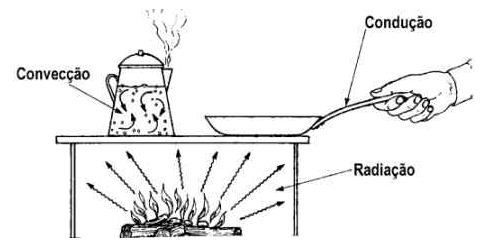
\includegraphics[width=8cm]{figuras/transferenciadecalor.png}
\caption{Mecanismos de transferência de calor}
\end{figure}

\section{Calorimetria}
A calorimetria é o estudo do calor como energia térmica em trânsito. Com dois corpos em temperaturas diferentes, a transmissão ocorre do corpo mais quente para o mais frio até atingirem o equilíbrio térmico. Uma das medidas mais usadas é a quantidade de calor (Q), ao receber energia térmica, essa quantidade de calor é positiva, ao perder é negativa.

\subsection{Calor Sensível e Latente}
Um corpo pode receber dois tipos de calor, o latente e o sensível. O calor latente é obtido quando o corpo muda de estado físico por causa dessa transferência, já o calor sensível é apenas mudança na temperatura do corpo.

Podemos representar seus cálculos com a fórmula fundamental da calorimetria e a equação para calcular o calor latente. Que são:

\begin{align}
Q_S=m \cdot c \cdot \Delta T
\end{align}
\begin{align}
Q_L=m \cdot L
\end{align}

Onde:
\begin{itemize}
\item $Q_S$ = Quantidade de calor sensível (em joules)
\item m = Massa do corpo em gramas
\item c = Calor sensível
\item $\Delta$T = Diferença de temperatura em ºC
\item $Q_L$ = Quantidade de calor Latente (em joules)
\item L = Constante de calor latente
\end{itemize}

	\section{Sistemas de Refrigeração}
	A área de refrigeração se desenvolveu de uma maneira extraordinária no último século, o que ocasionou sua atuação nos mais diversos campos da indústria. Para fins de estudos, as aplicações da refrigeração podem ser classificadas da seguinte forma: doméstica, comercial, industrial, para transporte e para condicionamento de ar. A primeira, refrigeração doméstica, abrange principalmente a fabricação de refrigeradores de uso doméstico e de freezers. A capacidade destes refrigeradores varia muito, mas se encontram na faixa de temperaturas entre $-8^oC$ a $-18^oC$ (no compartimento dos congelados) e $+2^oC$ a $+7^oC$ (no compartimento dos produtos resfriados).
	
	A refrigeração comercial envolve os refrigeradores especiais ou de grande porte utilizados principalmente em restaurantes, sorveterias, bares, açougues, laboratórios, entre outros. As suas temperaturas de congelamento e estocagem, são geralmente entre $-5^oC$ e $-30^oC$. 
	
	Os equipamentos industriais, em sua maioria, são maiores que os comerciais (com relação ao tamanho) e possuem como característica principal a necessidade de um operador de serviço. São exemplos de aplicações industriais as fábricas de gelo, grandes instalações de empacotamento de gêneros alimentícios, como carnes,peixes e aves, cervejarias, fábricas de laticínios, de processamento de bebidas, dentre outras.
	
	A refrigeração marítima é referente à refrigeração a bordo de embarcações e inclui, por exemplo, a refrigeração realizada em barcos de pesca e em embarcações de transporte de cargas perecíveis. A refrigeração de transporte,  por outro lado, envolve equipamentos de refrigeração para caminhões e vagões ferroviários refrigerados.
	
	Como se pode analisar, as aplicações na área da refrigeração são bem variadas, sendo difícil de uma certa maneira estabelecer de forma precisa as barreiras de cada uma dessas divisões.
	
		\subsection{Sistema de Compressão Mecânica de Vapor (CMV)}
		O sistema de compressão mecânica de vapor, utilizado na maioria dos sistemas de refrigeração atual, inclusive nos refrigeradores domésticos, funciona a partir da aplicação dos conceitos de calor e trabalho, utilizando um fluido refrigerante. Este fluido é uma substância que, circulando dentro de um circuito fechado, tem a capacidade de retirar o calor de um meio ao mesmo tempo em que se vaporiza em baixa pressão. O fluido entra no evaporador a baixa pressão, na forma de mistura de líquido-vapor, e retira energia do meio interno refrigerado (energia dos alimentos) enquanto passa para o seu estado de vapor. O vapor entra no compressor onde é comprimido e bombeado, transformando-se em vapor superaquecido e movimentando-se para o condensador, que possui a função de liberar a  energia retirado dos alimentos e resultante do trabalho de compressão para o meio exterior. O fluido, ao liberar essa energia, passa do estado de vapor superaquecido para líquido, ou seja ocorre o processo de condensação, e finalmente entra no dispositivo de expansão, onde a sua pressão é reduzida, para novamente ingressar no evaporador e reiniciar o ciclo. Esse processo é ilustrado na figura a seguir (Fig. \ref{geladeira}):
		
		\begin{figure}[H]
		\begin{center}
			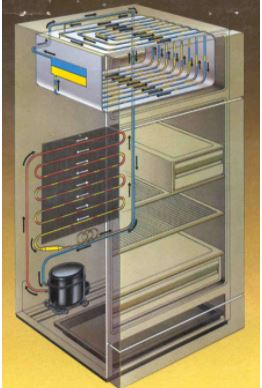
\includegraphics[scale =0.75]{figuras/Geladeira}
			\caption{Modelo de um CMV} \label{geladeira}
		\end{center}
		\end{figure}
			
	
	Os principais componentes desse sistema e suas funções estão definidas a seguir:
	
	\begin{itemize}
		\item  \textbf{COMPRESSOR:} Sua principal função é succionar o fluido refrigerante a baixa pressão da linha de sucção e comprimí-lo em direção ao condensador a alta pressão e temperatura na fase gasosa (vapor superaquecido).
			\begin{figure}[H]
				\begin{center}
					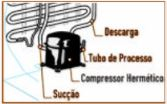
\includegraphics[scale =1]{figuras/Compressor}
					\caption{Modelo de um compressor}
				\end{center}
			\end{figure}	
		\item  \textbf{CONDENSADOR:} Por meio do condensador e suas aletas, o fluido refrigerante advindo do compressor a alta temperatura, efetua a troca de calor com o ambiente externo, liberando o calor que foi absorvido no evaporador e no processo de compressão. Nesta etapa, ocorre uma transformação de vapor superaquecido para líquido sub resfriado a alta pressão.
		
		\begin{figure}[H]
			\begin{center}
				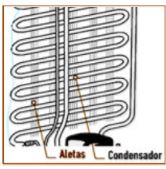
\includegraphics[scale =1]{figuras/Condensador}
				\caption{Modelo de um condensador}
			\end{center}
		\end{figure}
		\item  \textbf{FILTRO SECADOR:} Executa duas funções muito importantes: A primeira é reter as partículas sólidas que em circulação no circuito, podem provocar obstruções ou danos ao componentes mecânicos do compressor. A segunda é absorver totalmente a umidade residual do circuito que ocasionalmente não tenha sido retirada pelo processo de vácuo, poupando danos ao sistema, como por exemplo, a formação de ácidos, corrosão, aumento das pressões de trabalho e obstrução do tubo capilar por congelamento das gotículas de umidade.
			\begin{figure}[H]
				\begin{center}
					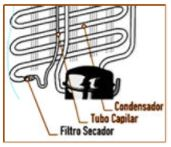
\includegraphics[scale =1]{figuras/filtro_secador}
					\caption{Modelo de um filtro secador}
				\end{center}
			\end{figure}
		
		\item  \textbf{TUBO CAPILAR:} É um tubo de cobre com o diâmetro reduzido que tem como finalidade receber o fluido refrigerante do condensador e proporcionar a perda de carga do fluido refrigerante separando os lados de alta e baixa pressão.
		
		\item  \textbf{EVAPORADOR:} Recepciona o fluido refrigerante proveniente do tubo capilar, em seu estado líquido a baixa pressão e temperatura. Desta forma, o fluido evapora absorvendo o calor da superfície da tubulação do evaporador, ocorrendo a transformação de líquido sub resfriado para vapor saturado a baixa pressão. Este efeito ocasiona a diminuição de temperatura do ambiente interno do refrigerador.
					\begin{figure}[H]
						\begin{center}
							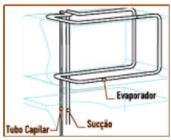
\includegraphics[scale=1]{figuras/Evaporador.JPG}
							\caption{Modelo de um evaporador}
						\end{center}
					\end{figure}
					
			\end{itemize}
	
		De forma parecida funcionam também os grandes sistemas de refrigeração, como as câmaras frigoríficas por exemplo. O que difere entre esses sistemas é o número de unidades compressoras, evaporadoras, de expansão e condensadoras compreendidas, que nestes últimos podem ser múltiplos, bem como o sistema de controle que pode se tornar altamente complexo.
	